% Latex template: mahmoud.s.fahmy@students.kasralainy.edu.eg
% For more details: https://www.sharelatex.com/learn/Beamer

\documentclass{beamer}					% Document class
\geometry{papersize={15cm,10cm}}

\setbeamertemplate{footline}[text line]{%
  \parbox{\linewidth}{\vspace*{-8pt}\hfill\hfill\insertpagenumber}}
\setbeamertemplate{navigation symbols}{}

\usepackage[english]{babel}				% Set language
\usepackage[utf8x]{inputenc}			% Set encoding

\mode<presentation>						% Set options
{
  \usetheme{default}					% Set theme
  \usecolortheme{default} 				% Set colors
  \usefonttheme{default}  				% Set font theme
  \setbeamertemplate{caption}[numbered]	% Set caption to be numbered
}

% Uncomment this to have the outline at the beginning of each section highlighted.
%\AtBeginSection[]
%{
%  \begin{frame}{Outline}
%    \tableofcontents[currentsection]
%  \end{frame}
\usepackage{graphicx}					% For including figures
\usepackage{booktabs}					% For table rules
\usepackage{hyperref}	
\usepackage{tikz-network}				% For cross-referencing
\usepackage[absolute,overlay]{textpos}
\usepackage{bm}
\usepackage[font=small,labelfont=bf]{caption}				% For cross-referencing

\title{Visualizing nucleosome cluster dynamics with dense single molecule localization microscopy}	% Presentation title
\author{Clayton W. Seitz}								% Presentation author
\date{\today}									% Today's date	

\begin{document}

% Title page
% This page includes the informations defined earlier including title, author/s, affiliation/s and the date
\begin{frame}
  \titlepage
\end{frame}


% The following is the most frequently used slide types in beamer
% The slide structure is as follows:
%
%\begin{frame}{<slide-title>}
%	<content>
%\end{frame}


\begin{frame}
\begin{itemize}
\item Overview of biological system and some literature review
\item Open questions in that system
\item A novel method to study that system
\item Major results so far
\item Future goals and perspectives
\end{itemize}
\end{frame}


\begin{frame}{The textbook view of histone acetylation}
\begin{figure}
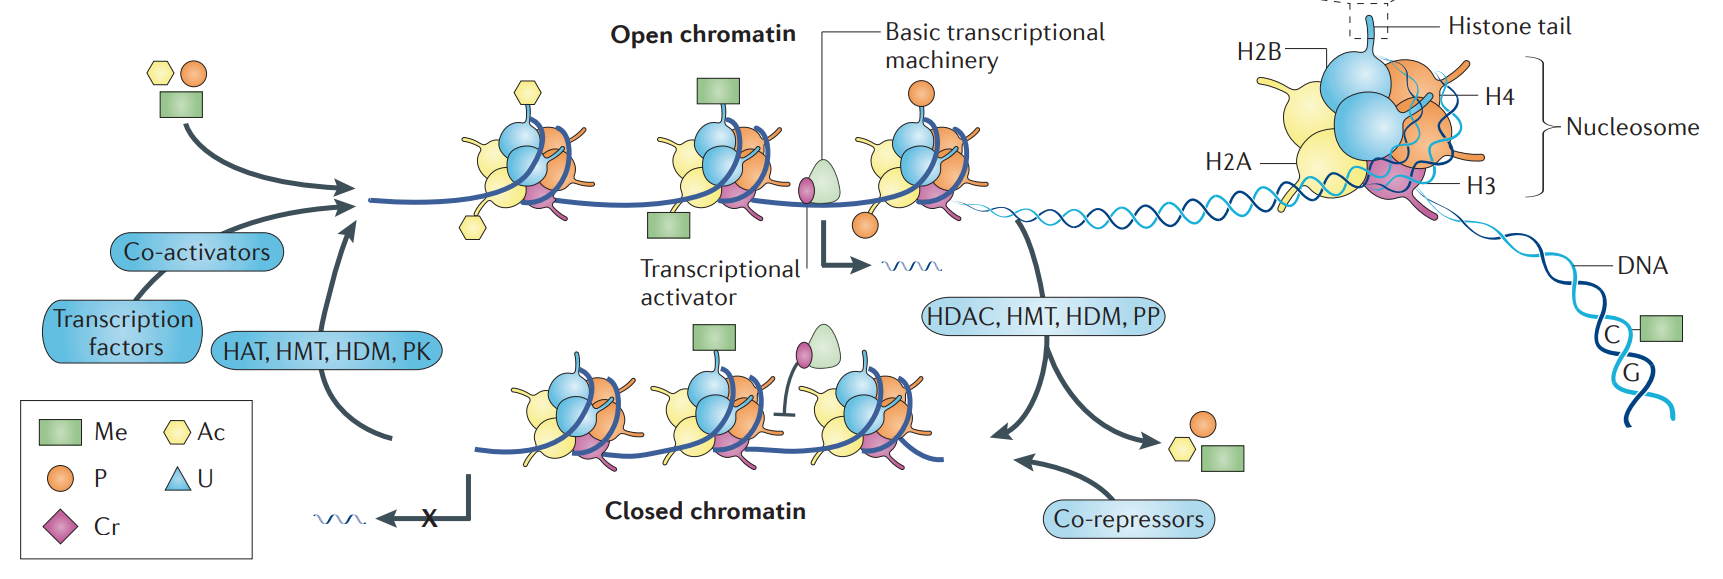
\includegraphics[width=13cm]{Histones.png}
\end{figure}
\textit{Graff et al. Histone acetylation: molecular
mnemonics on the chromatin}
\vspace{0.1in}
\begin{itemize}
\item I am interested in the impact of BRD4 protein on chromatin structure
\item Previous work has shown BRD4 is associated with histone acetylation
\item Live cell super-resolution imaging is a useful tool
\end{itemize}
\end{frame}

\begin{frame}{A phase separation model for transcriptional control}
\begin{figure}
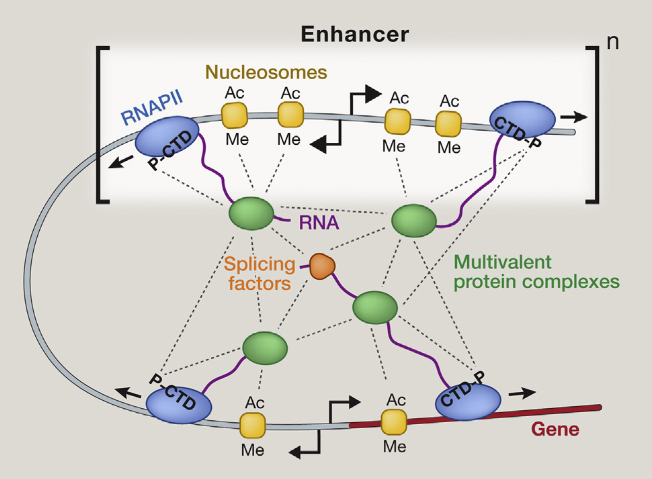
\includegraphics[width=10cm]{Super1.png}
\end{figure}
\textit{Hnisz et al. A phase separation model of transcriptional control. Cell 2017}
\end{frame}

\begin{frame}{A phase separation model for transcriptional control}
\begin{figure}
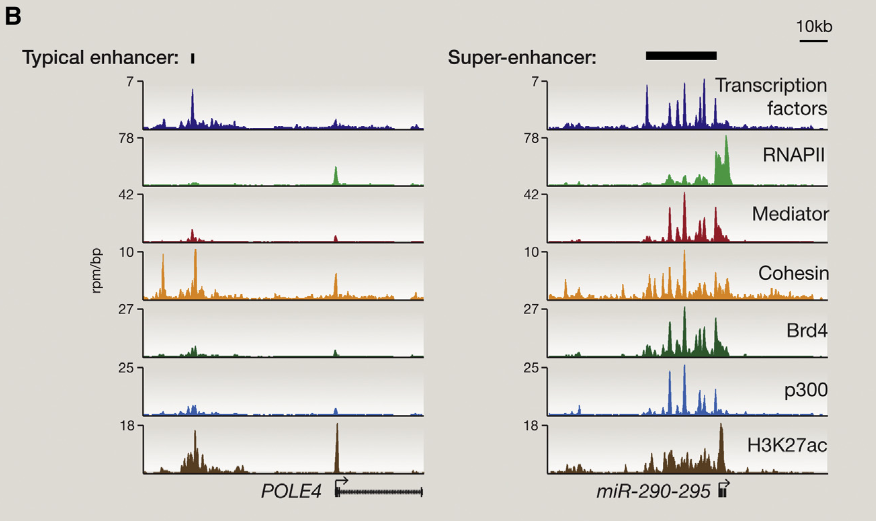
\includegraphics[width=11cm]{Super2.png}
\end{figure}
\textit{Hnisz et al. A phase separation model of transcriptional control. Cell 2017}
\end{frame}

\begin{frame}{(+)-JQ1 in complex with BRD4 protein}

\begin{textblock*}{6cm}(1.0cm,1.5cm)
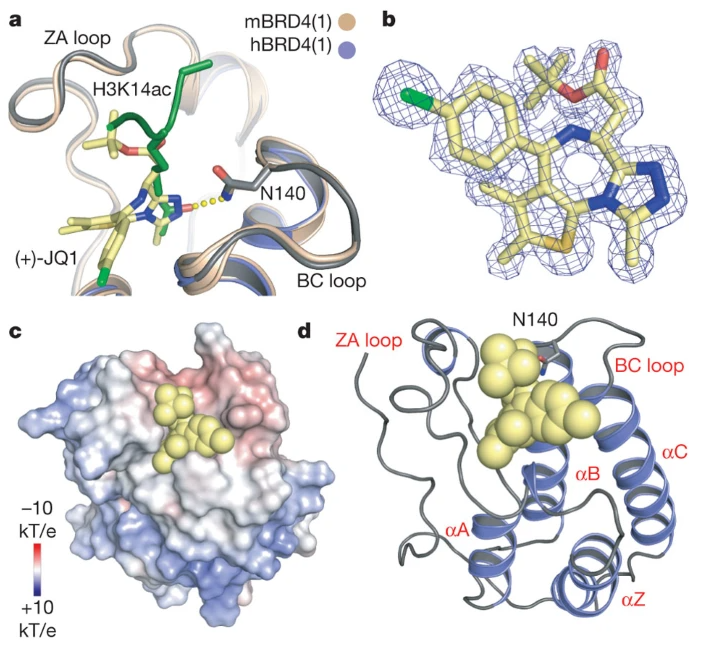
\includegraphics[width=6cm]{JQ1_Complex.png}
\end{textblock*}

\begin{textblock*}{8cm}(7.5cm,1.75cm)
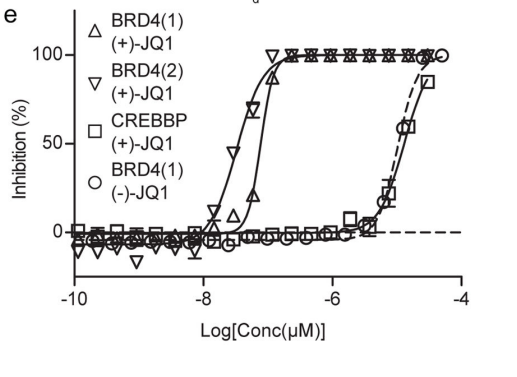
\includegraphics[width=8cm]{BRD4-Inhibition.png}
\end{textblock*}

\begin{textblock*}{\textwidth}(1.0cm,8cm)
\textit{Filippakopoulos. Selective inhibition of BET bromodomains. Nature Communications}

\end{textblock*}


\end{frame}

\begin{frame}{Validaton of JQ1 efficacy for BRD4 inhibition in Hela cells}

\begin{figure}
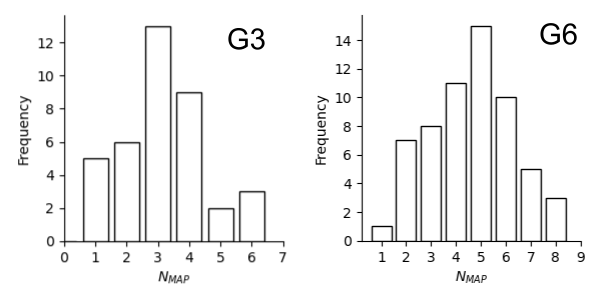
\includegraphics[width=12cm]{Figure-5.png}
\end{figure}

\begin{itemize}
\item RT-qPCR quantified using $2^{-\Delta\Delta C_{t}}$ method using GAPDH as a reference gene
\item *:$P \leq 0.1$, **:$P \leq 0.01$
\end{itemize}

\end{frame}

\begin{frame}{Induction of a BRD4-controlled gene with cytokine treatment}
\begin{figure}
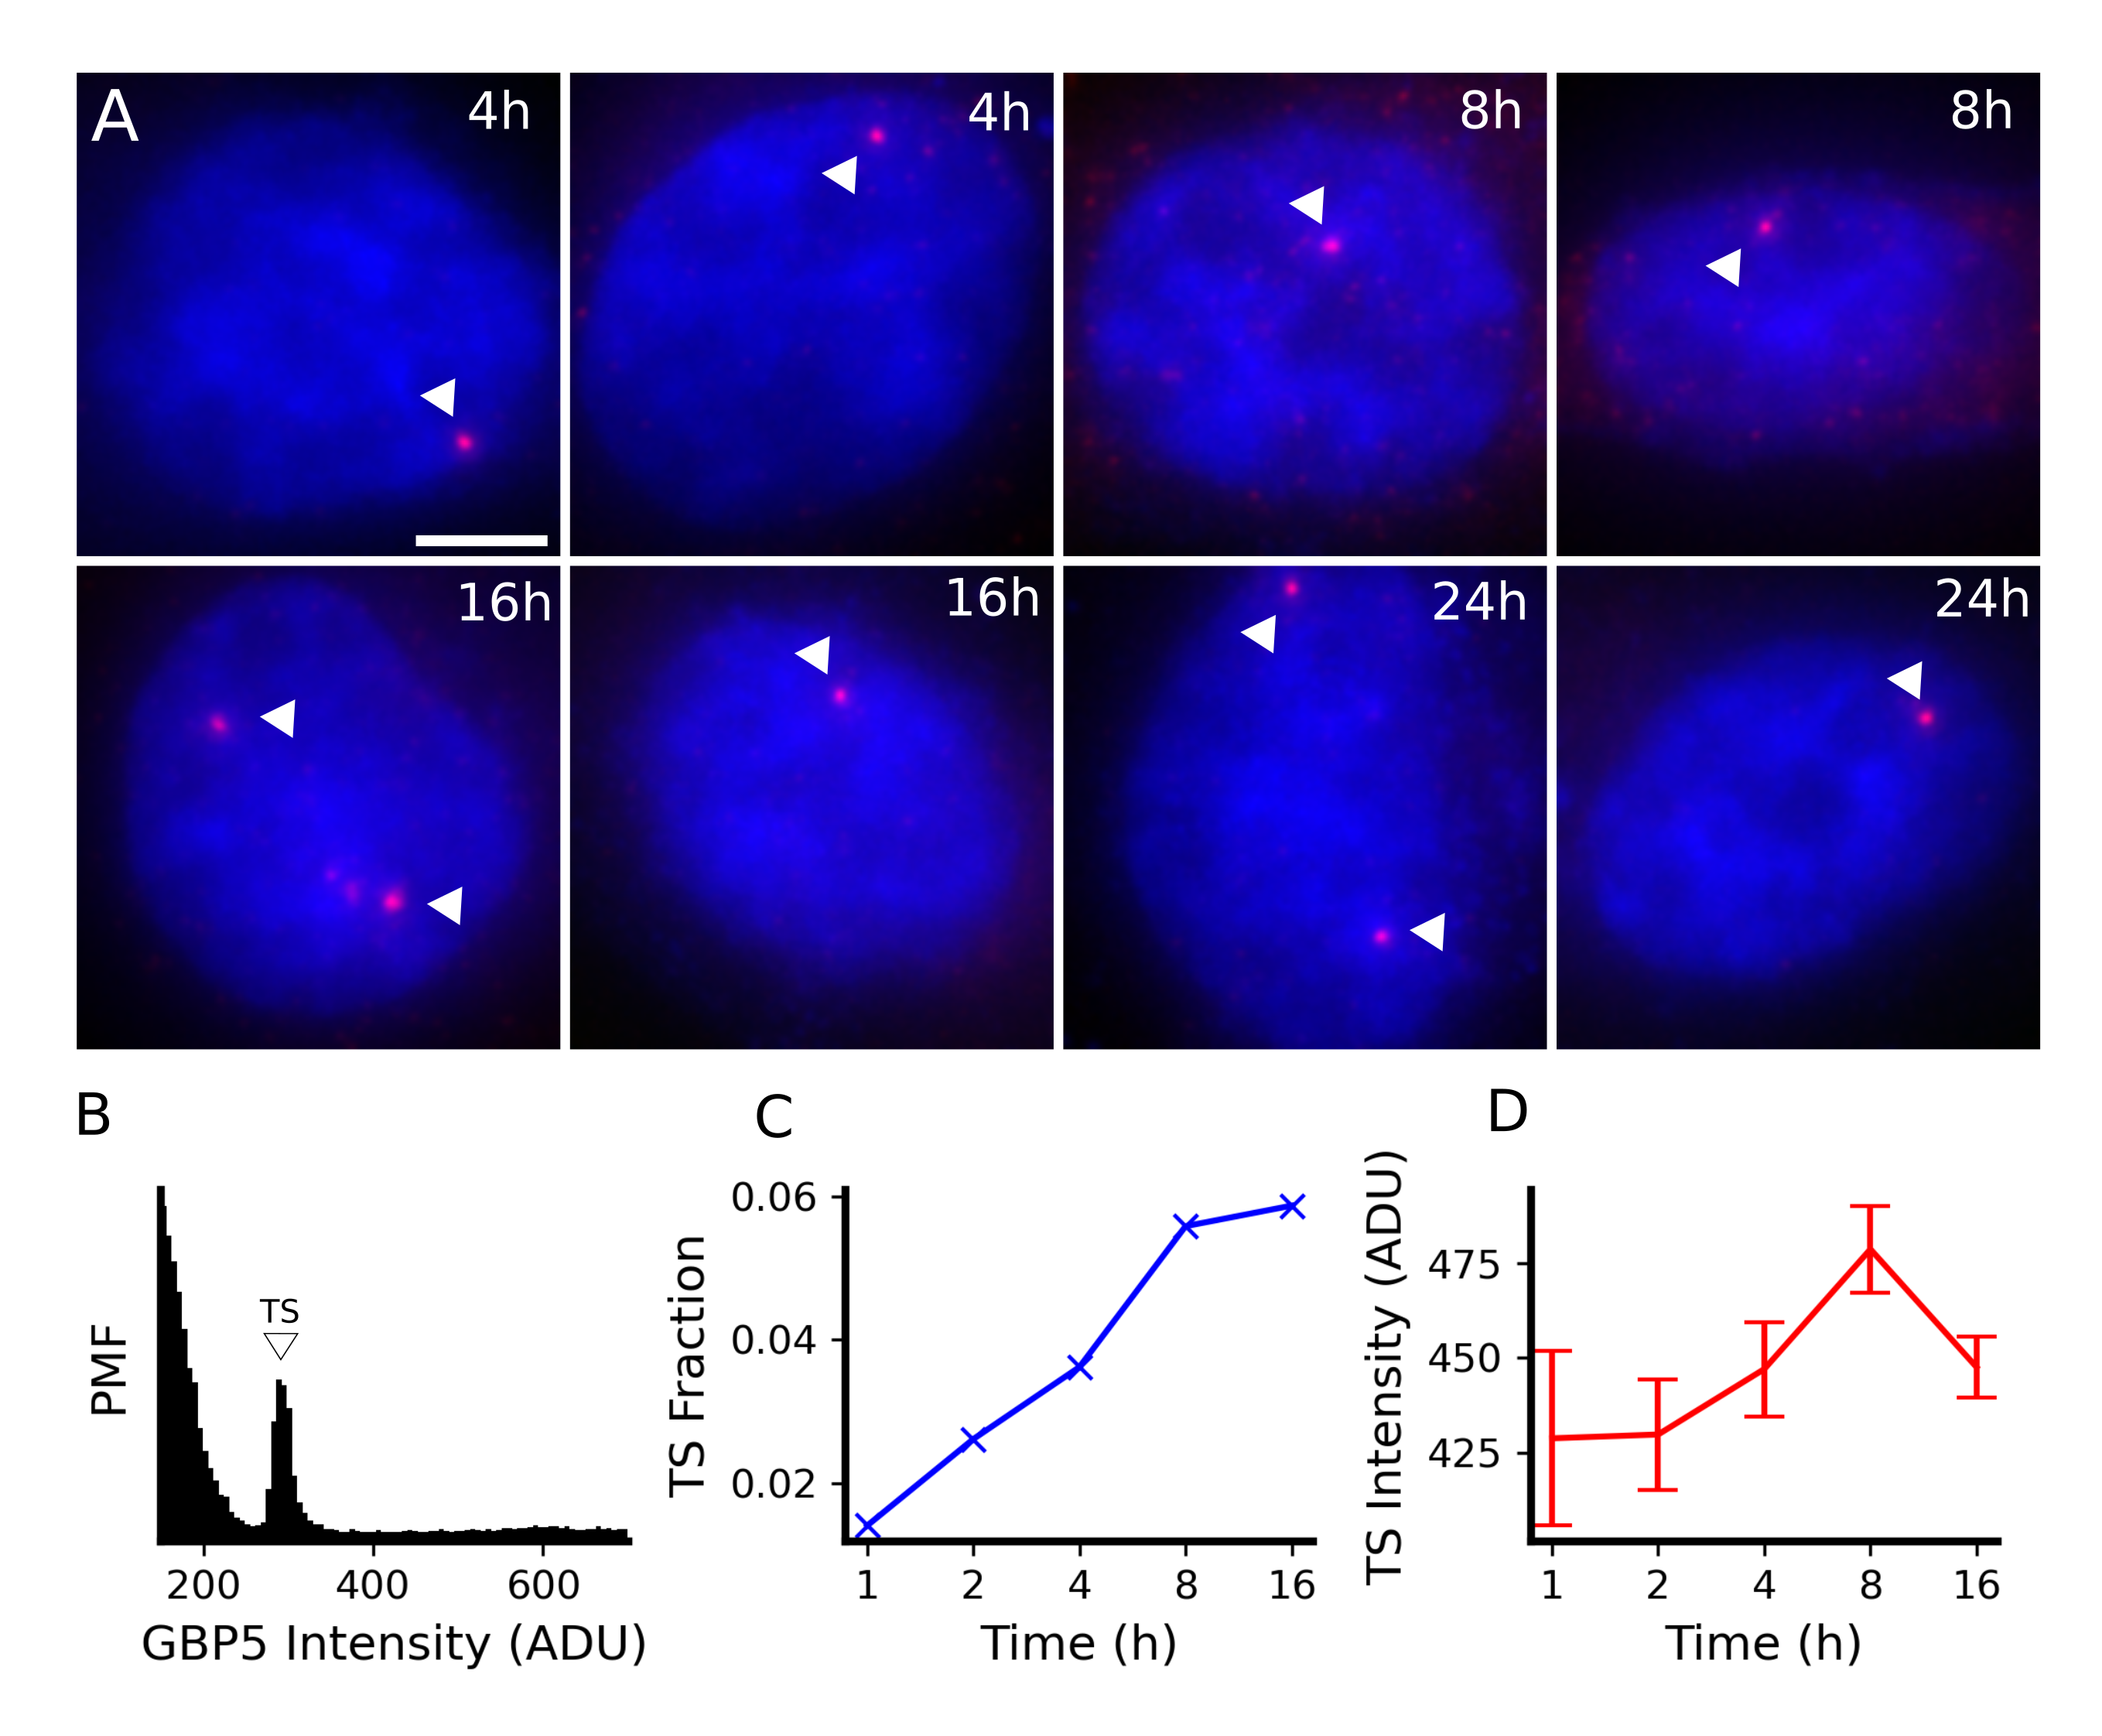
\includegraphics[width=11cm]{Figure-2.png}
\end{figure}
\begin{itemize}
\item GBP5 transcription is regulated by BRD4 (Lin 2022)
\end{itemize}
\end{frame}




\begin{frame}
\frametitle{Instrumentation for single molecule localization microscopy}

\begin{figure}
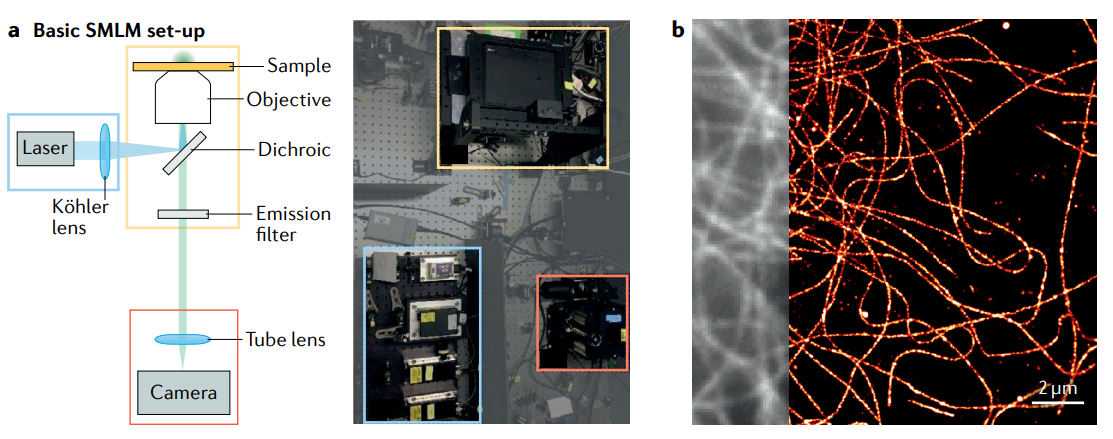
\includegraphics[width=12cm]{Setup.png}
\end{figure}

\end{frame}

\begin{frame}{A Poisson approximation at moderate SNR simplifies SMLM}

\begin{figure}
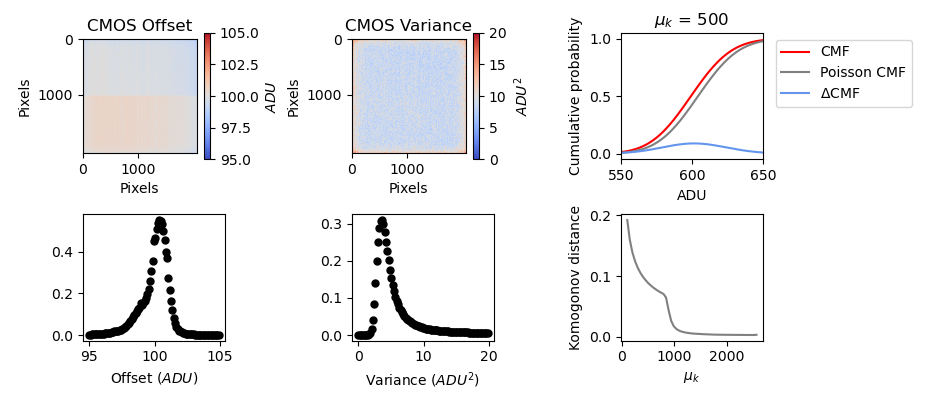
\includegraphics[width=13cm]{Noise.png}
\end{figure}

\begin{equation*}
P(H_{k}|\theta) = A\sum_{q=0}^{\infty} \frac{1}{q!}e^{-\mu_{k}}\mu_{k}^{q}\frac{1}{\sqrt{2\pi}\sigma_{k}}e^{-\frac{(H_{k}-g_{k}q-o_{k})}{2\sigma_{k}^{2}}}
\end{equation*}

$P(H_{k}|\theta)$ can be approximated as Poisson at high signal-to-noise ($\mathrm{SNR}$)
 
\end{frame}


\begin{frame}{Maximum likelihood localization of an isolated fluorescent emitter}
Localization: $\theta^{*} = \underset{\theta}{\mathrm{argmax}}\prod_{k}P(H_{k}|\theta)= \underset{\theta}{\mathrm{argmin}}-\sum_{k}\log P(H_{k}|\theta)$

\begin{textblock*}{8cm}(6.5cm,2.5cm)
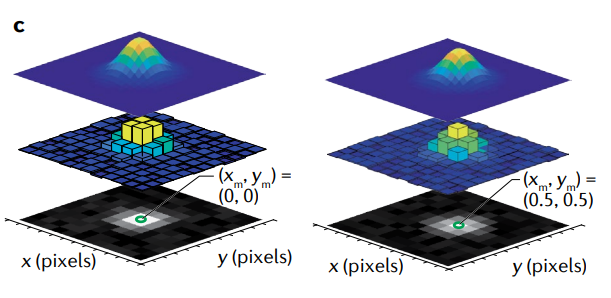
\includegraphics[width=\textwidth]{Model.png}
\end{textblock*}

\begin{textblock*}{2cm}(1cm,2.5cm)
\begin{align*}
\mu_{k} &= g_{k}\textcolor{red}{\eta} \textcolor{cyan}{N_{0}}\textcolor{blue}{\Delta}\int_{\mathrm{pixel}} G(x,y)dA\\
\\
\textcolor{red}{\eta} &- \mathrm{quantum\; efficiency}\\
\textcolor{cyan}{N_{0}} &- \mathrm{photon\; count}\\
\textcolor{blue}{\Delta} &- \mathrm{exposure\; time}
\end{align*}
\end{textblock*}


\vspace{2in}

\begin{itemize}
\item Fisher information and Cramer-Rao lower bound (CRLB) can be computed analytically for Poisson log-likelihood $\ell$ (Smith 2010, Huang 2013)
\end{itemize} 

\end{frame}



\begin{frame}{Estimator precision sets the resolution limit in localization microscopy}
\begin{textblock*}{4cm}(1.0cm,1.0cm)
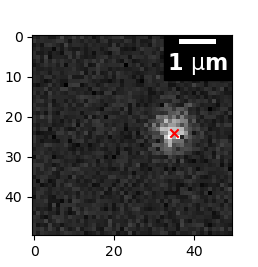
\includegraphics[width=4cm]{MCMC/Figure_1.png}
\end{textblock*}
\begin{textblock*}{4cm}(1.0cm,5cm)
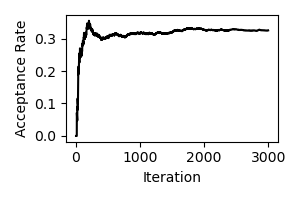
\includegraphics[width=4cm]{MCMC/Figure_2.png}
\end{textblock*}
\begin{textblock*}{9cm}(5cm,1.0cm)
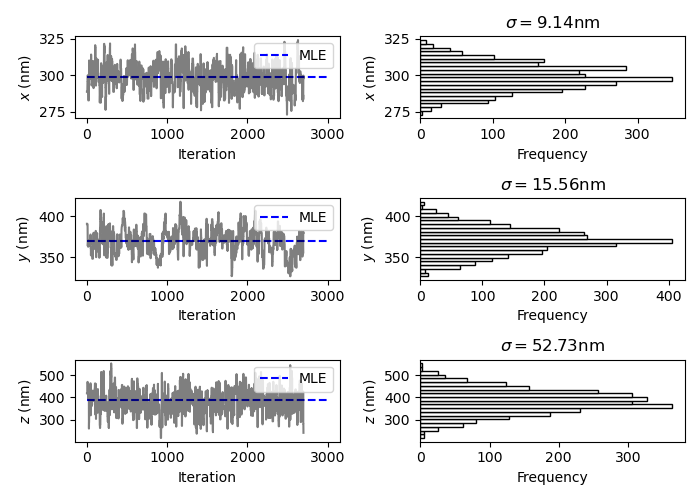
\includegraphics[width=9cm]{MCMC/Figure_3.png}
\end{textblock*}
\begin{textblock*}{13cm}(0.5cm,8cm)
\begin{itemize}
\item Variance of the posterior $P(\theta|\vec{H})$ is a useful particle filter
\item We assume uniform priors on coordinates
\end{itemize}
\end{textblock*}
\end{frame}

\begin{frame}{Computing the CRLB for static errors in two dimensions}
Fisher information (separable case): \begin{equation}
I_{ij}(\theta) = \underset{\theta}{\mathbb{E}}\left(\frac{\partial \ell}{\partial\theta_{i}}\frac{\partial\ell}{\partial\theta_{j}}\right) 
\end{equation}

Let $\mu_{k}' = \mu_{k} + \sigma_{k}^{2}$. For an arbitrary parameter,

\begin{align*}
\frac{\partial \ell}{\partial \theta_{i}} &= \frac{\partial}{\partial \theta_{i}} \sum_{k}  x_{k}\log x_{k} + \mu_{k}' - x_{k}\log\left(\mu_{k}'\right)\\
&= \sum_{k} \frac{\partial \mu_{k}'}{\partial\theta_{i}} \left(\frac{\mu_{k}'-x_{k}}{\mu_{k}'}\right)
\end{align*}

\begin{equation*}
I_{ij}(\theta) = \underset{\theta}{\mathbb{E}}\left(\sum_{k}\frac{\partial \mu_{k}'}{\partial\theta_{i}}\frac{\partial \mu_{k}'}{\partial\theta_{j}} \left(\frac{\mu_{k}'-x_{k}}{\mu_{k}'}\right)^{2}\right) = \sum_{k}\frac{1}{\mu_{k}'}\frac{\partial \mu_{k}'}{\partial\theta_{i}}\frac{\partial \mu_{k}'}{\partial\theta_{j}}
\end{equation*}
The CRLB is a frequentist 
\end{frame}

\begin{frame}
\frametitle{Direct STORM: The photophysics of rhodamines}

\begin{figure}
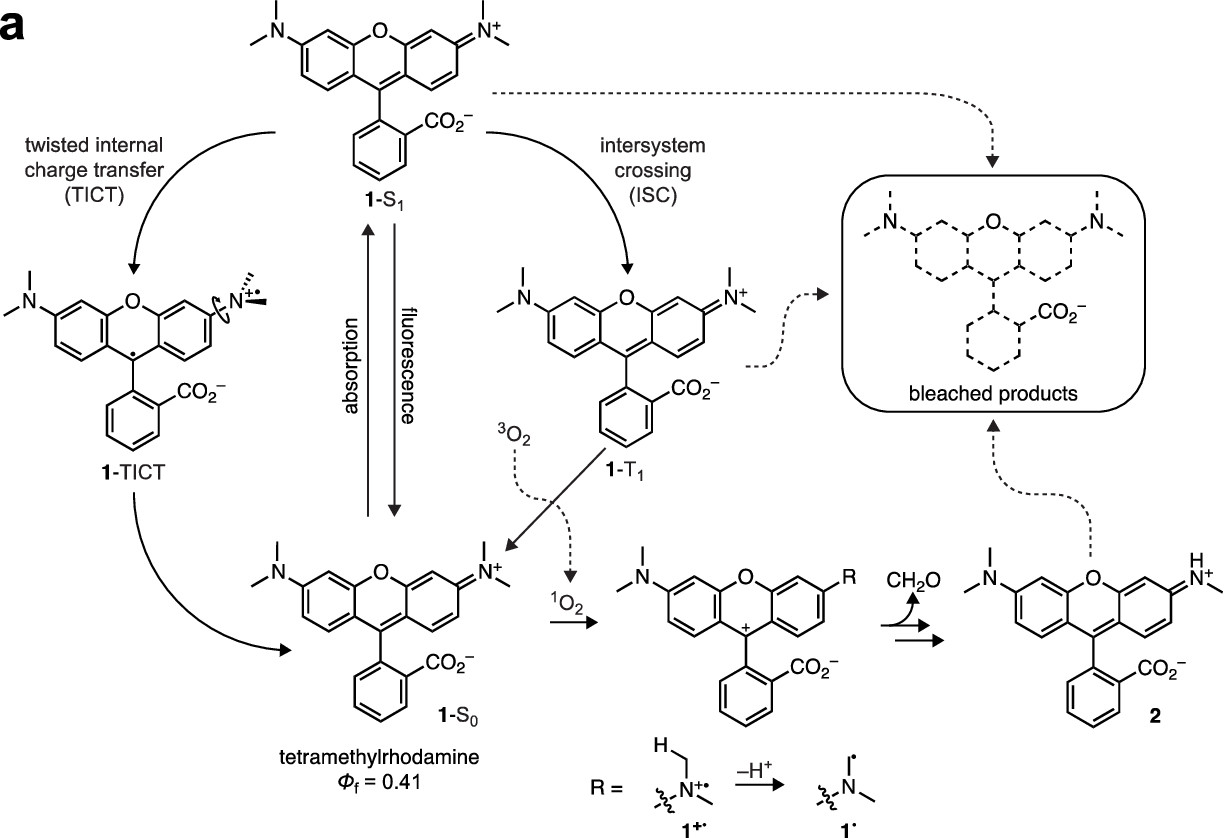
\includegraphics[width=10cm]{Rhodamines.png}
\end{figure}
\begin{itemize}
\item  Reduction of the T1 state yields a dark, long-lived, and stable radical state
\item The reducing agent is usually a primary thiol like cysteamine (MEA)
\end{itemize}
\end{frame}

\begin{frame}{The OFF state of JF646 can be maintained with high laser power}
\begin{textblock*}{11cm}(1.5cm,1.3cm)
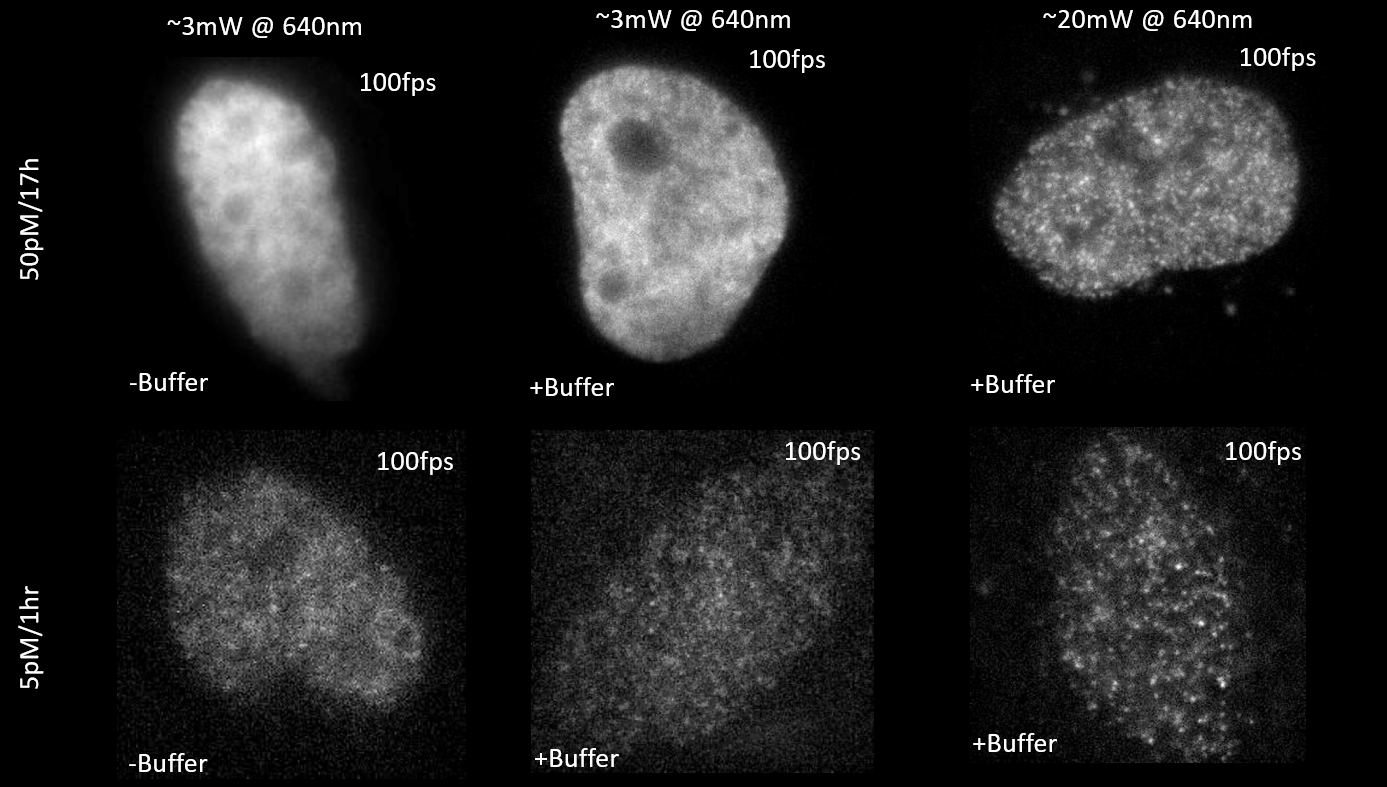
\includegraphics[width=11cm]{Laser.png}
\end{textblock*}
\begin{textblock*}{\textwidth}(0.5cm,8.0cm)
\begin{itemize}
\item High power maintains the OFF state, potentially by promoting triplet state formation
\end{itemize}
\end{textblock*}
\end{frame}

\begin{frame}{The tradeoff between spatial and temporal resolution in SMLM}
\begin{textblock*}{10cm}(2.25cm,1.25cm)
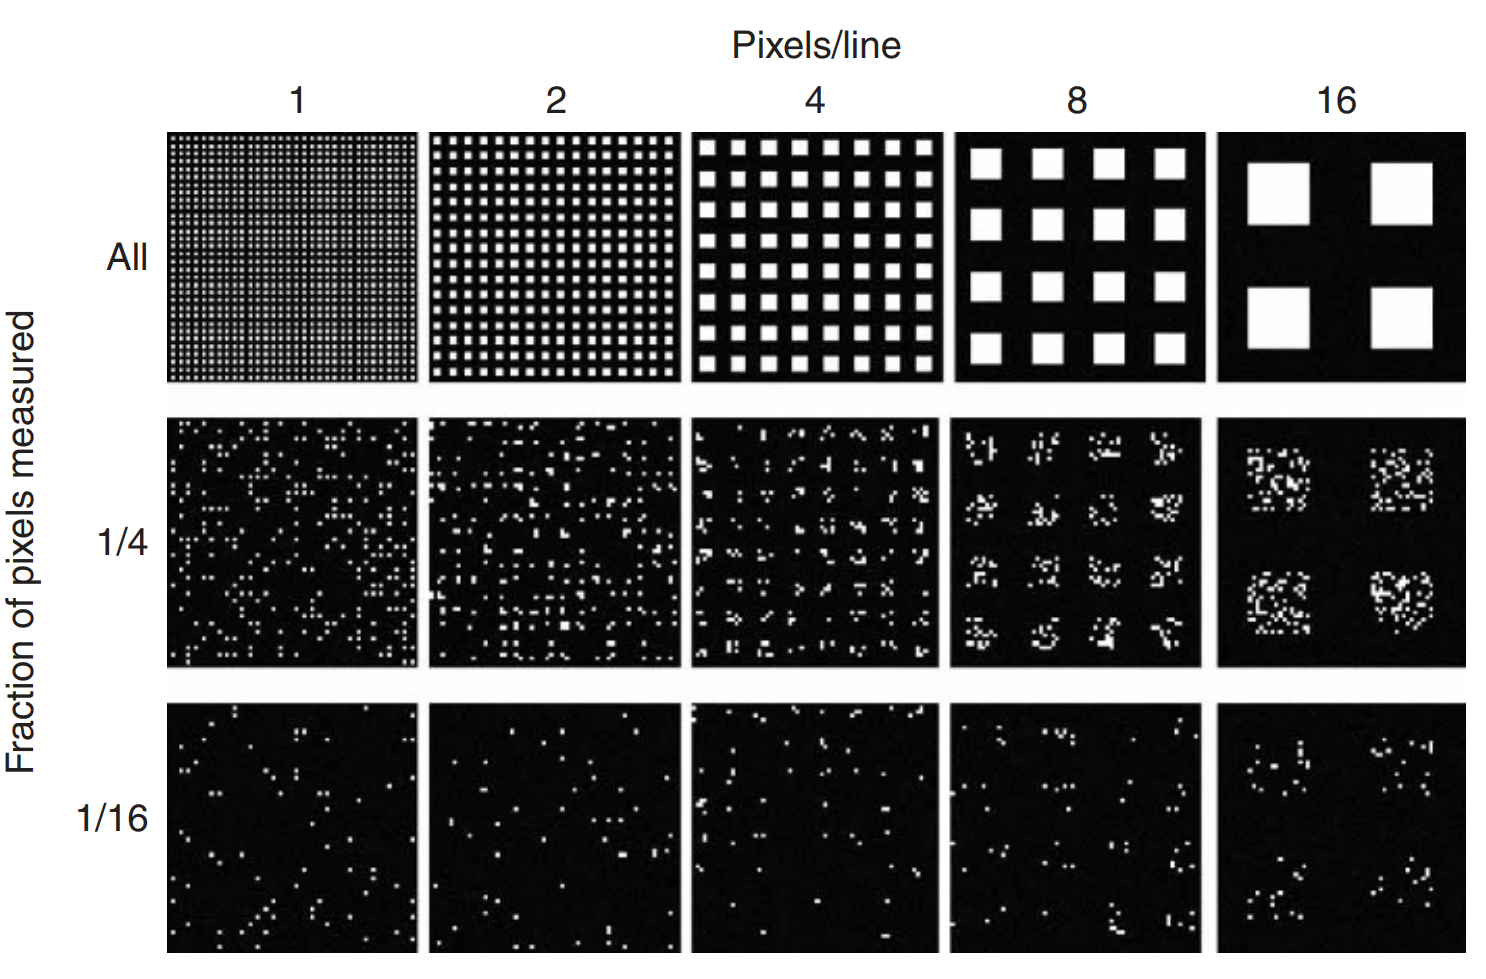
\includegraphics[width=10cm]{Shroff.png}
\end{textblock*}
\begin{textblock*}{\textwidth}(0.5cm,8.0cm)
\begin{itemize}
\item SMLM is desirable for SR due to very high res and no scanning (e.g., STED)
\item Less control over photophysical state, but high throughput
\end{itemize}
\end{textblock*}
\end{frame}




\begin{frame}{Deep learning enables dense localization in two-dimensions}
\begin{textblock*}{10cm}(4.25cm,1.25cm)
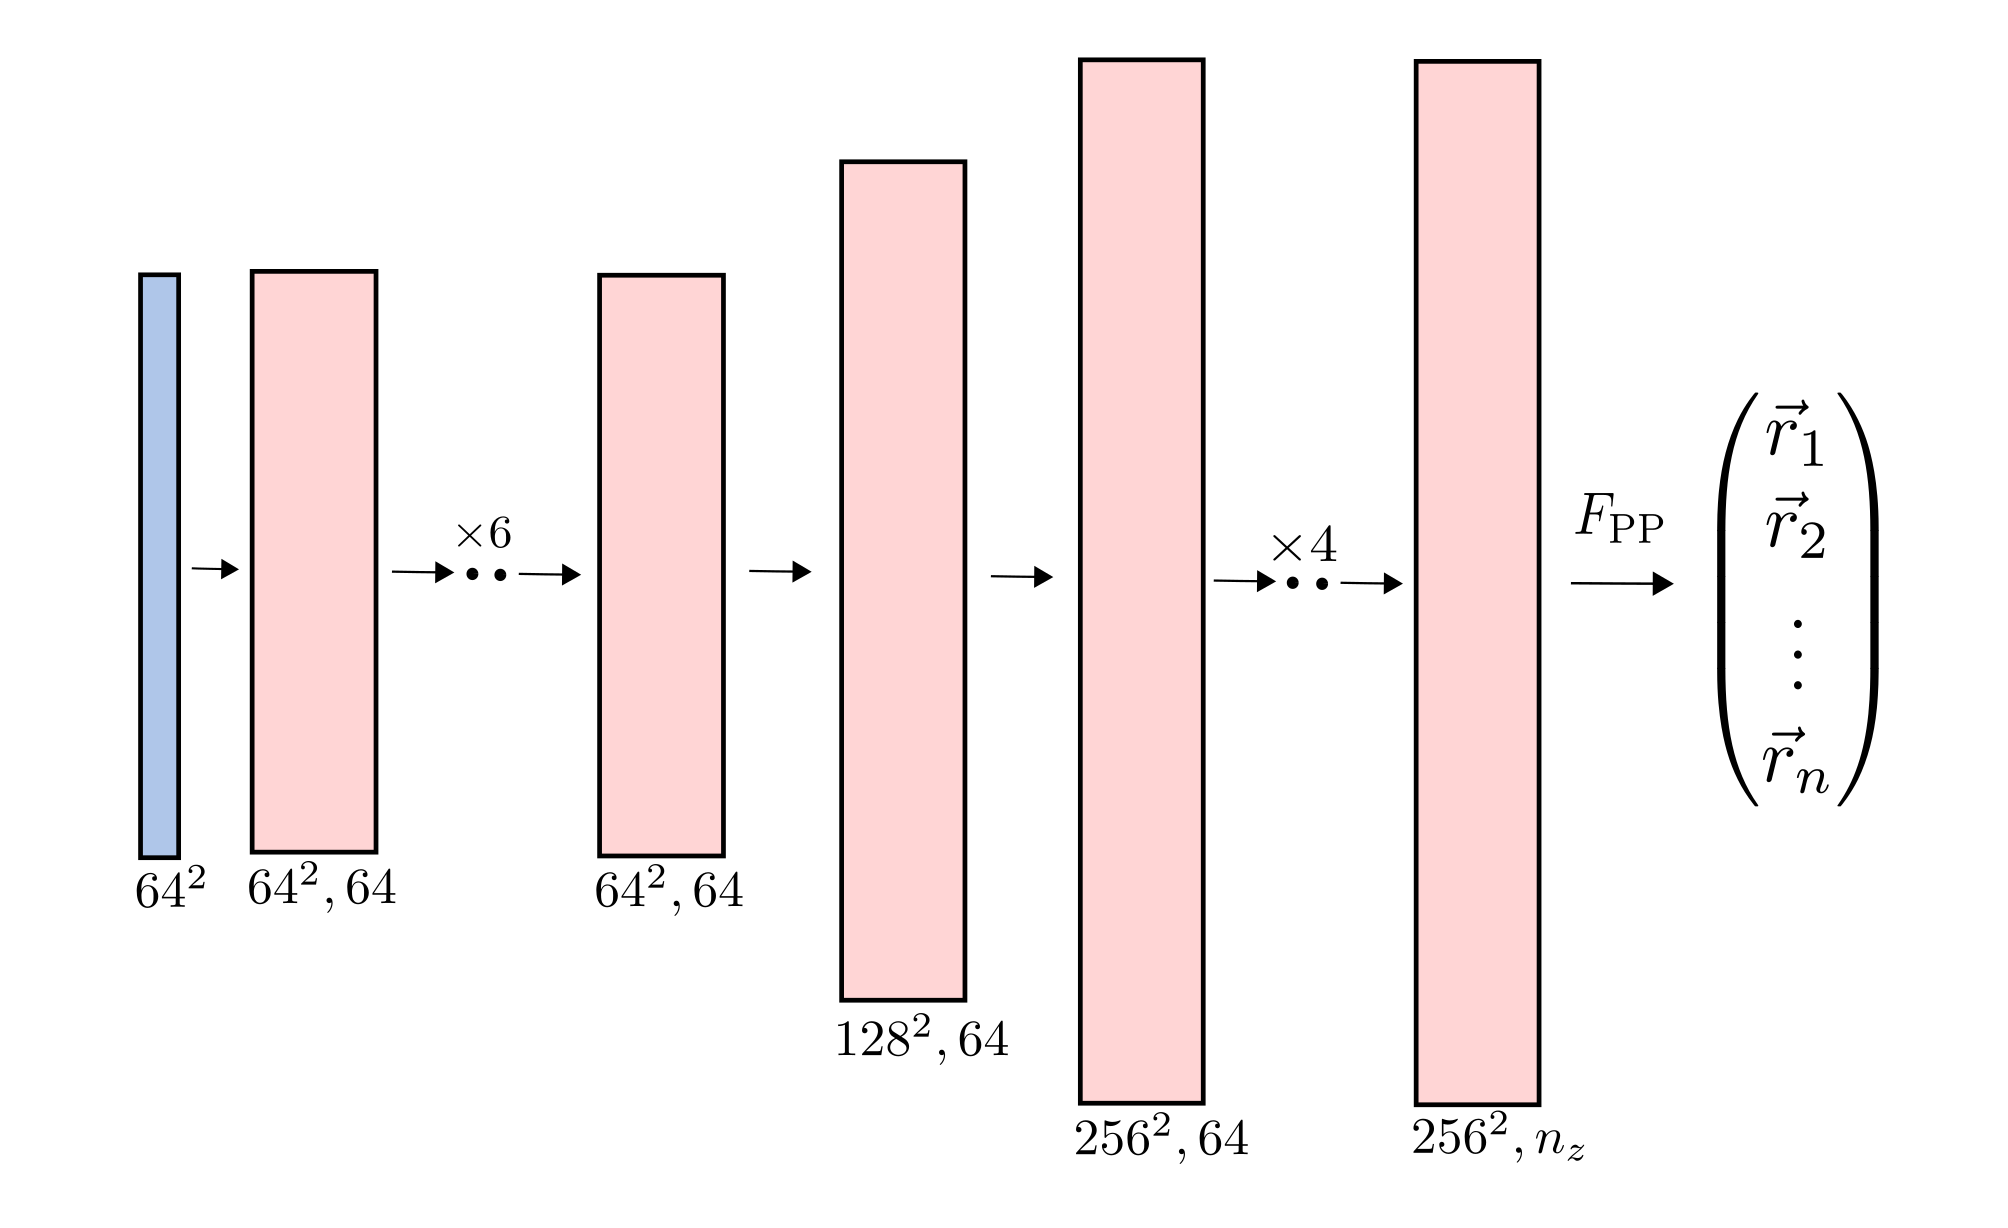
\includegraphics[width=10cm]{DeepSTORM.png}
\end{textblock*}
\begin{textblock*}{2.5cm}(1.5cm,2.75cm)
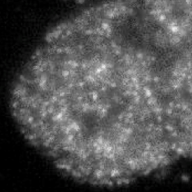
\includegraphics[width=2.5cm]{Laser-Crop.png}
\end{textblock*}

\begin{textblock*}{\textwidth}(1cm,7.5cm)

Localization is cast as semantic segmentation of the high resolution tensor:

\begin{equation*}
\mathcal{L} = \sum_{i,j} \log p_{ij}(\tilde{x}) = \sum_{i,j} \log \frac{\exp(-s_{ij}(\tilde{x}))}{\sum_{x\in\chi} \exp(-s_{ij}(\tilde{x}))}
\end{equation*}

\end{textblock*}

\end{frame}


\begin{frame}{Estimator precision sets the resolution limit in localization microscopy}

\begin{textblock*}{18cm}(1.25cm,1.5cm)
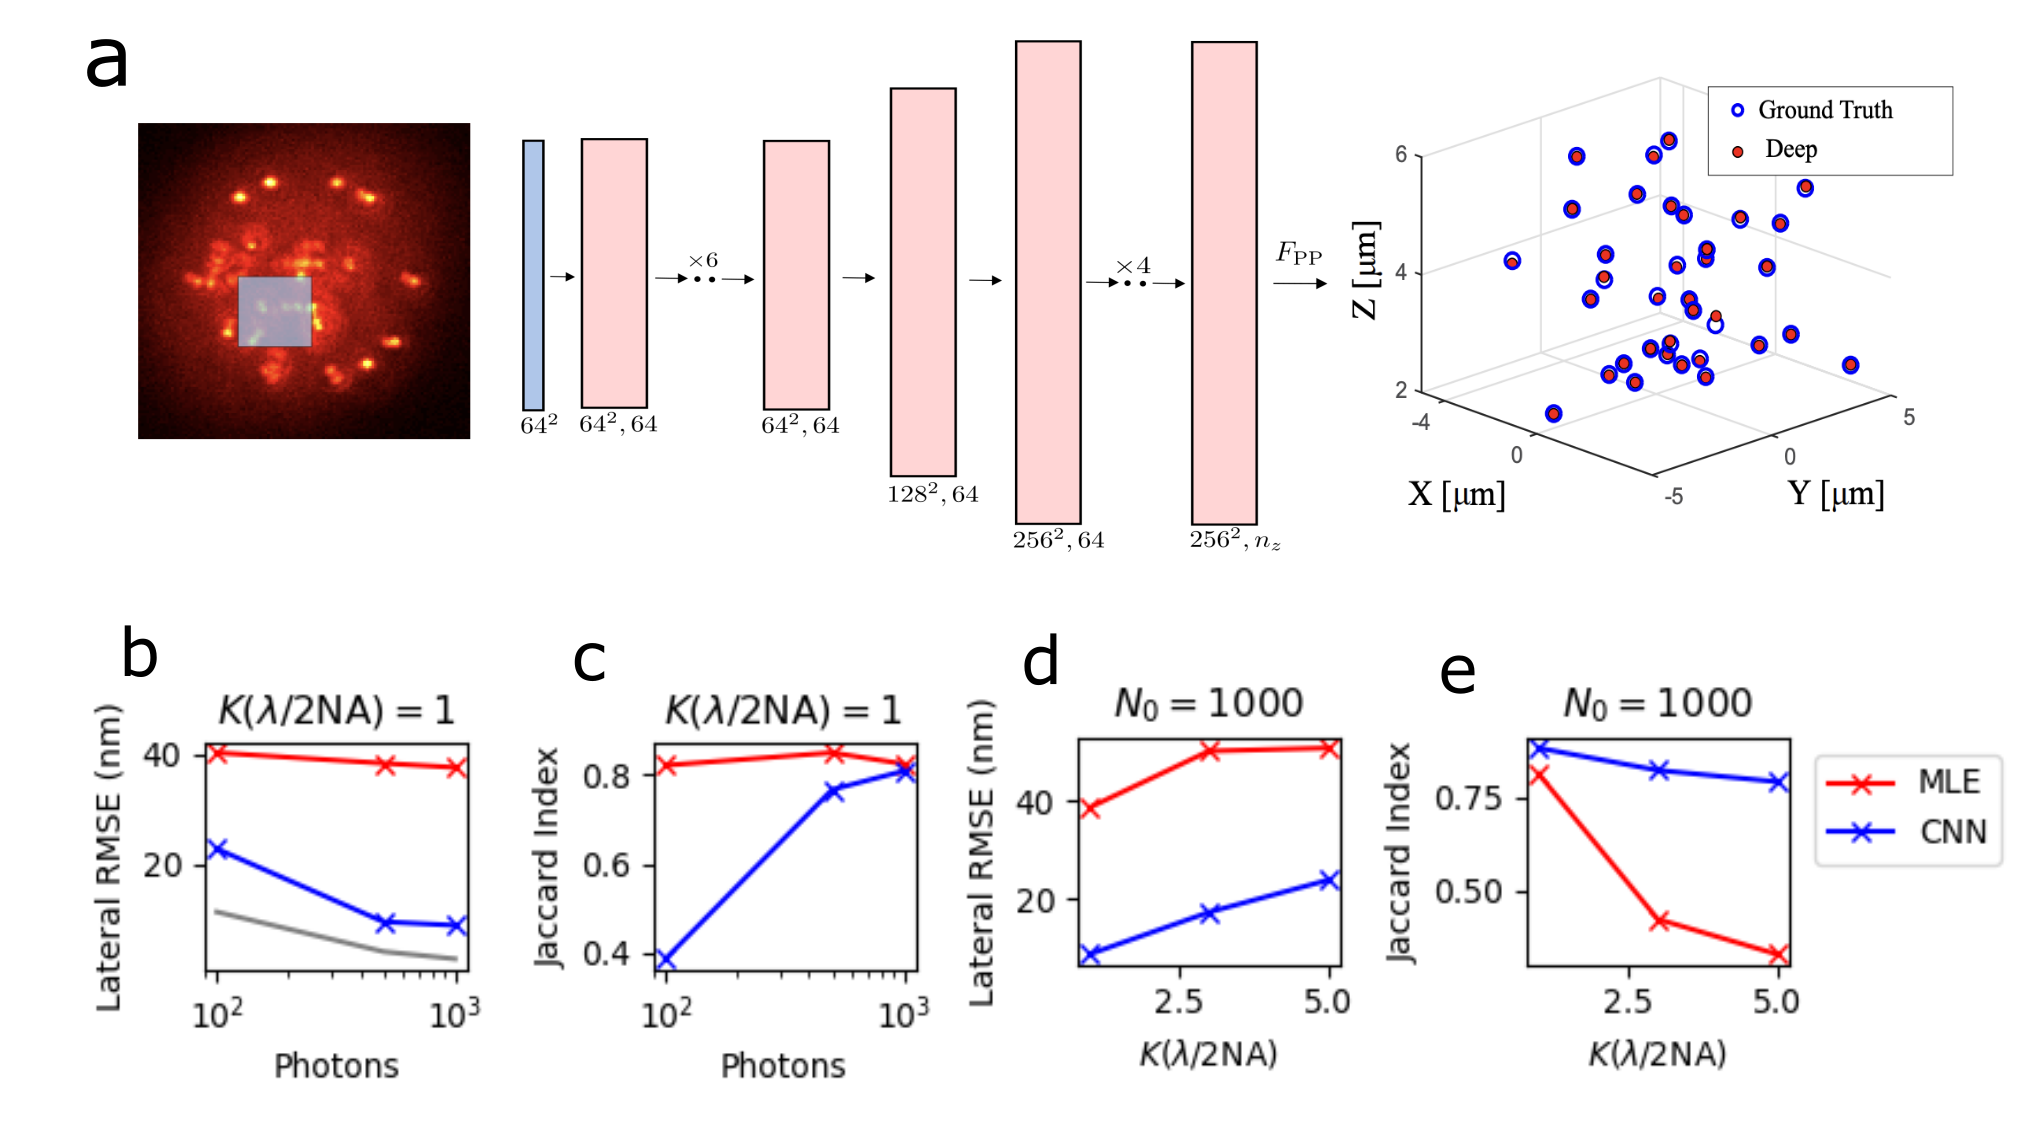
\includegraphics[width=10cm]{PSF2D.png}
\end{textblock*}

\end{frame}

\begin{frame}{Estimator precision sets the resolution limit in localization microscopy}

\begin{textblock*}{10cm}(1.25cm,1.5cm)
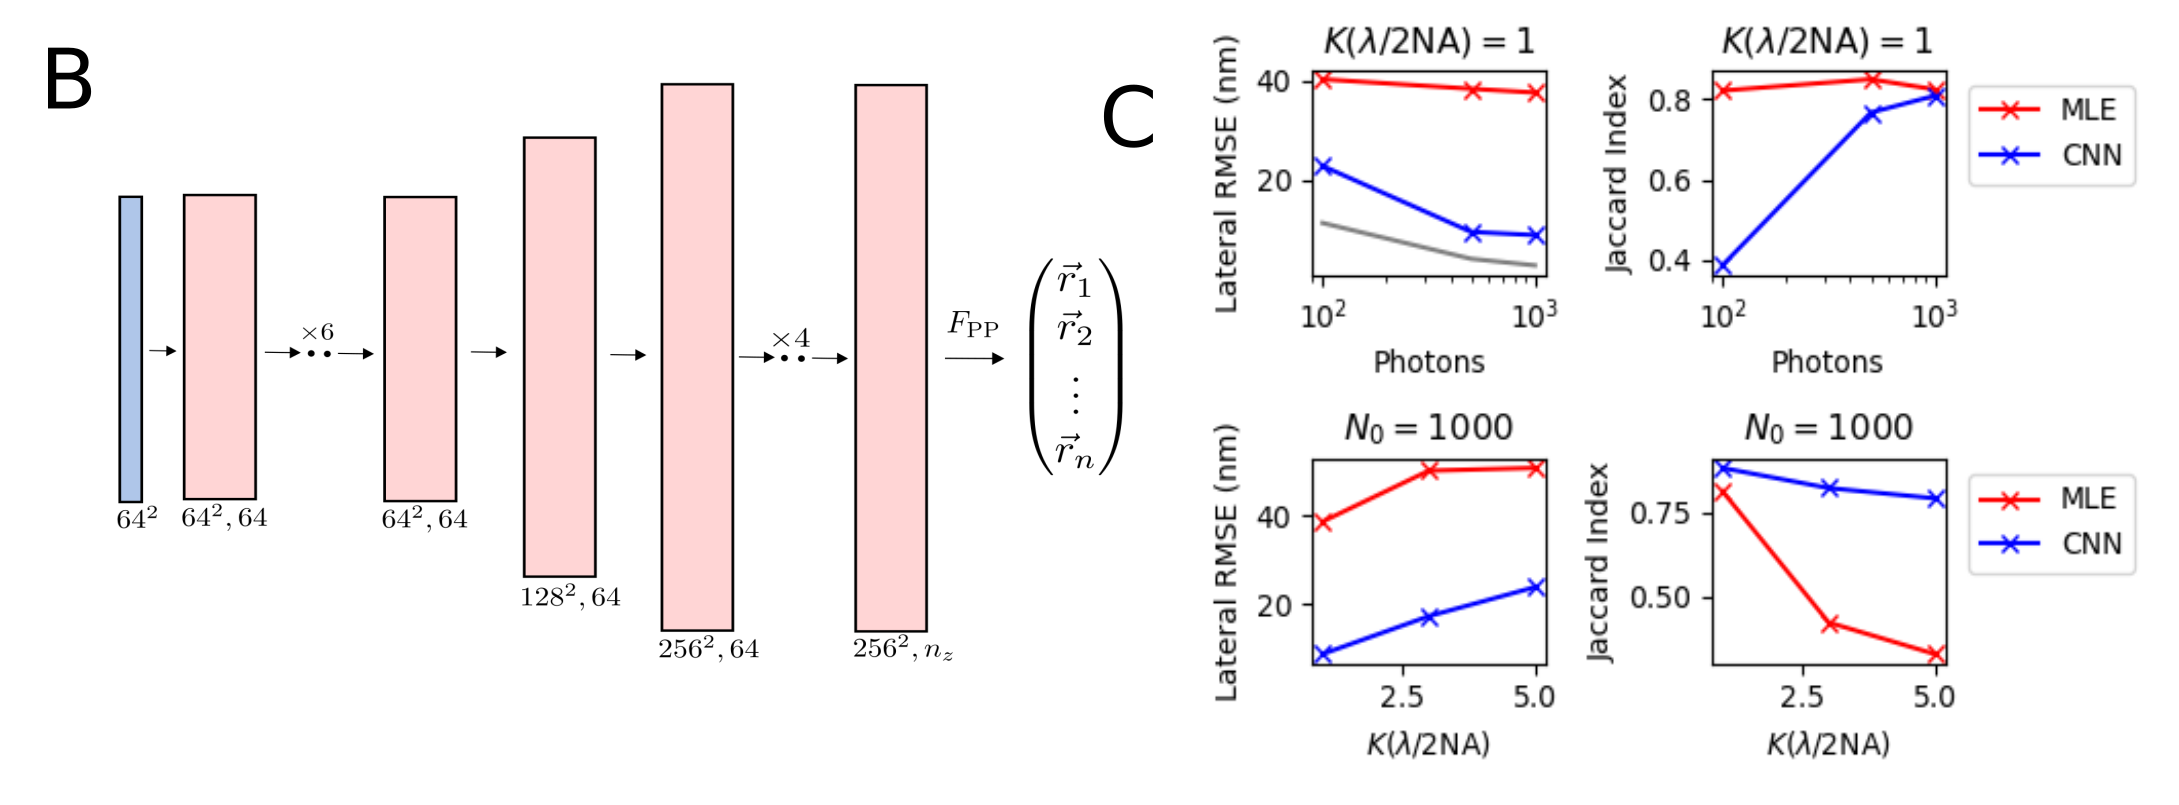
\includegraphics[width=13cm]{PSF2D-Crop.png}
\end{textblock*}
\begin{textblock*}{13cm}(1.25cm,7cm)
\begin{itemize}
\item $K(\lambda/2\mathrm{NA})$ is Ripley's K function at the diffraction limit ($\lambda=640\mathrm{nm}$)
\item Convolutional neural networks (CNNs) approach the CRLB (gray) at high photon counts and generalize to the dense regime
\end{itemize}
\end{textblock*}

\end{frame}


\begin{frame}{Astigmatism based three dimensional imaging}
\begin{figure}
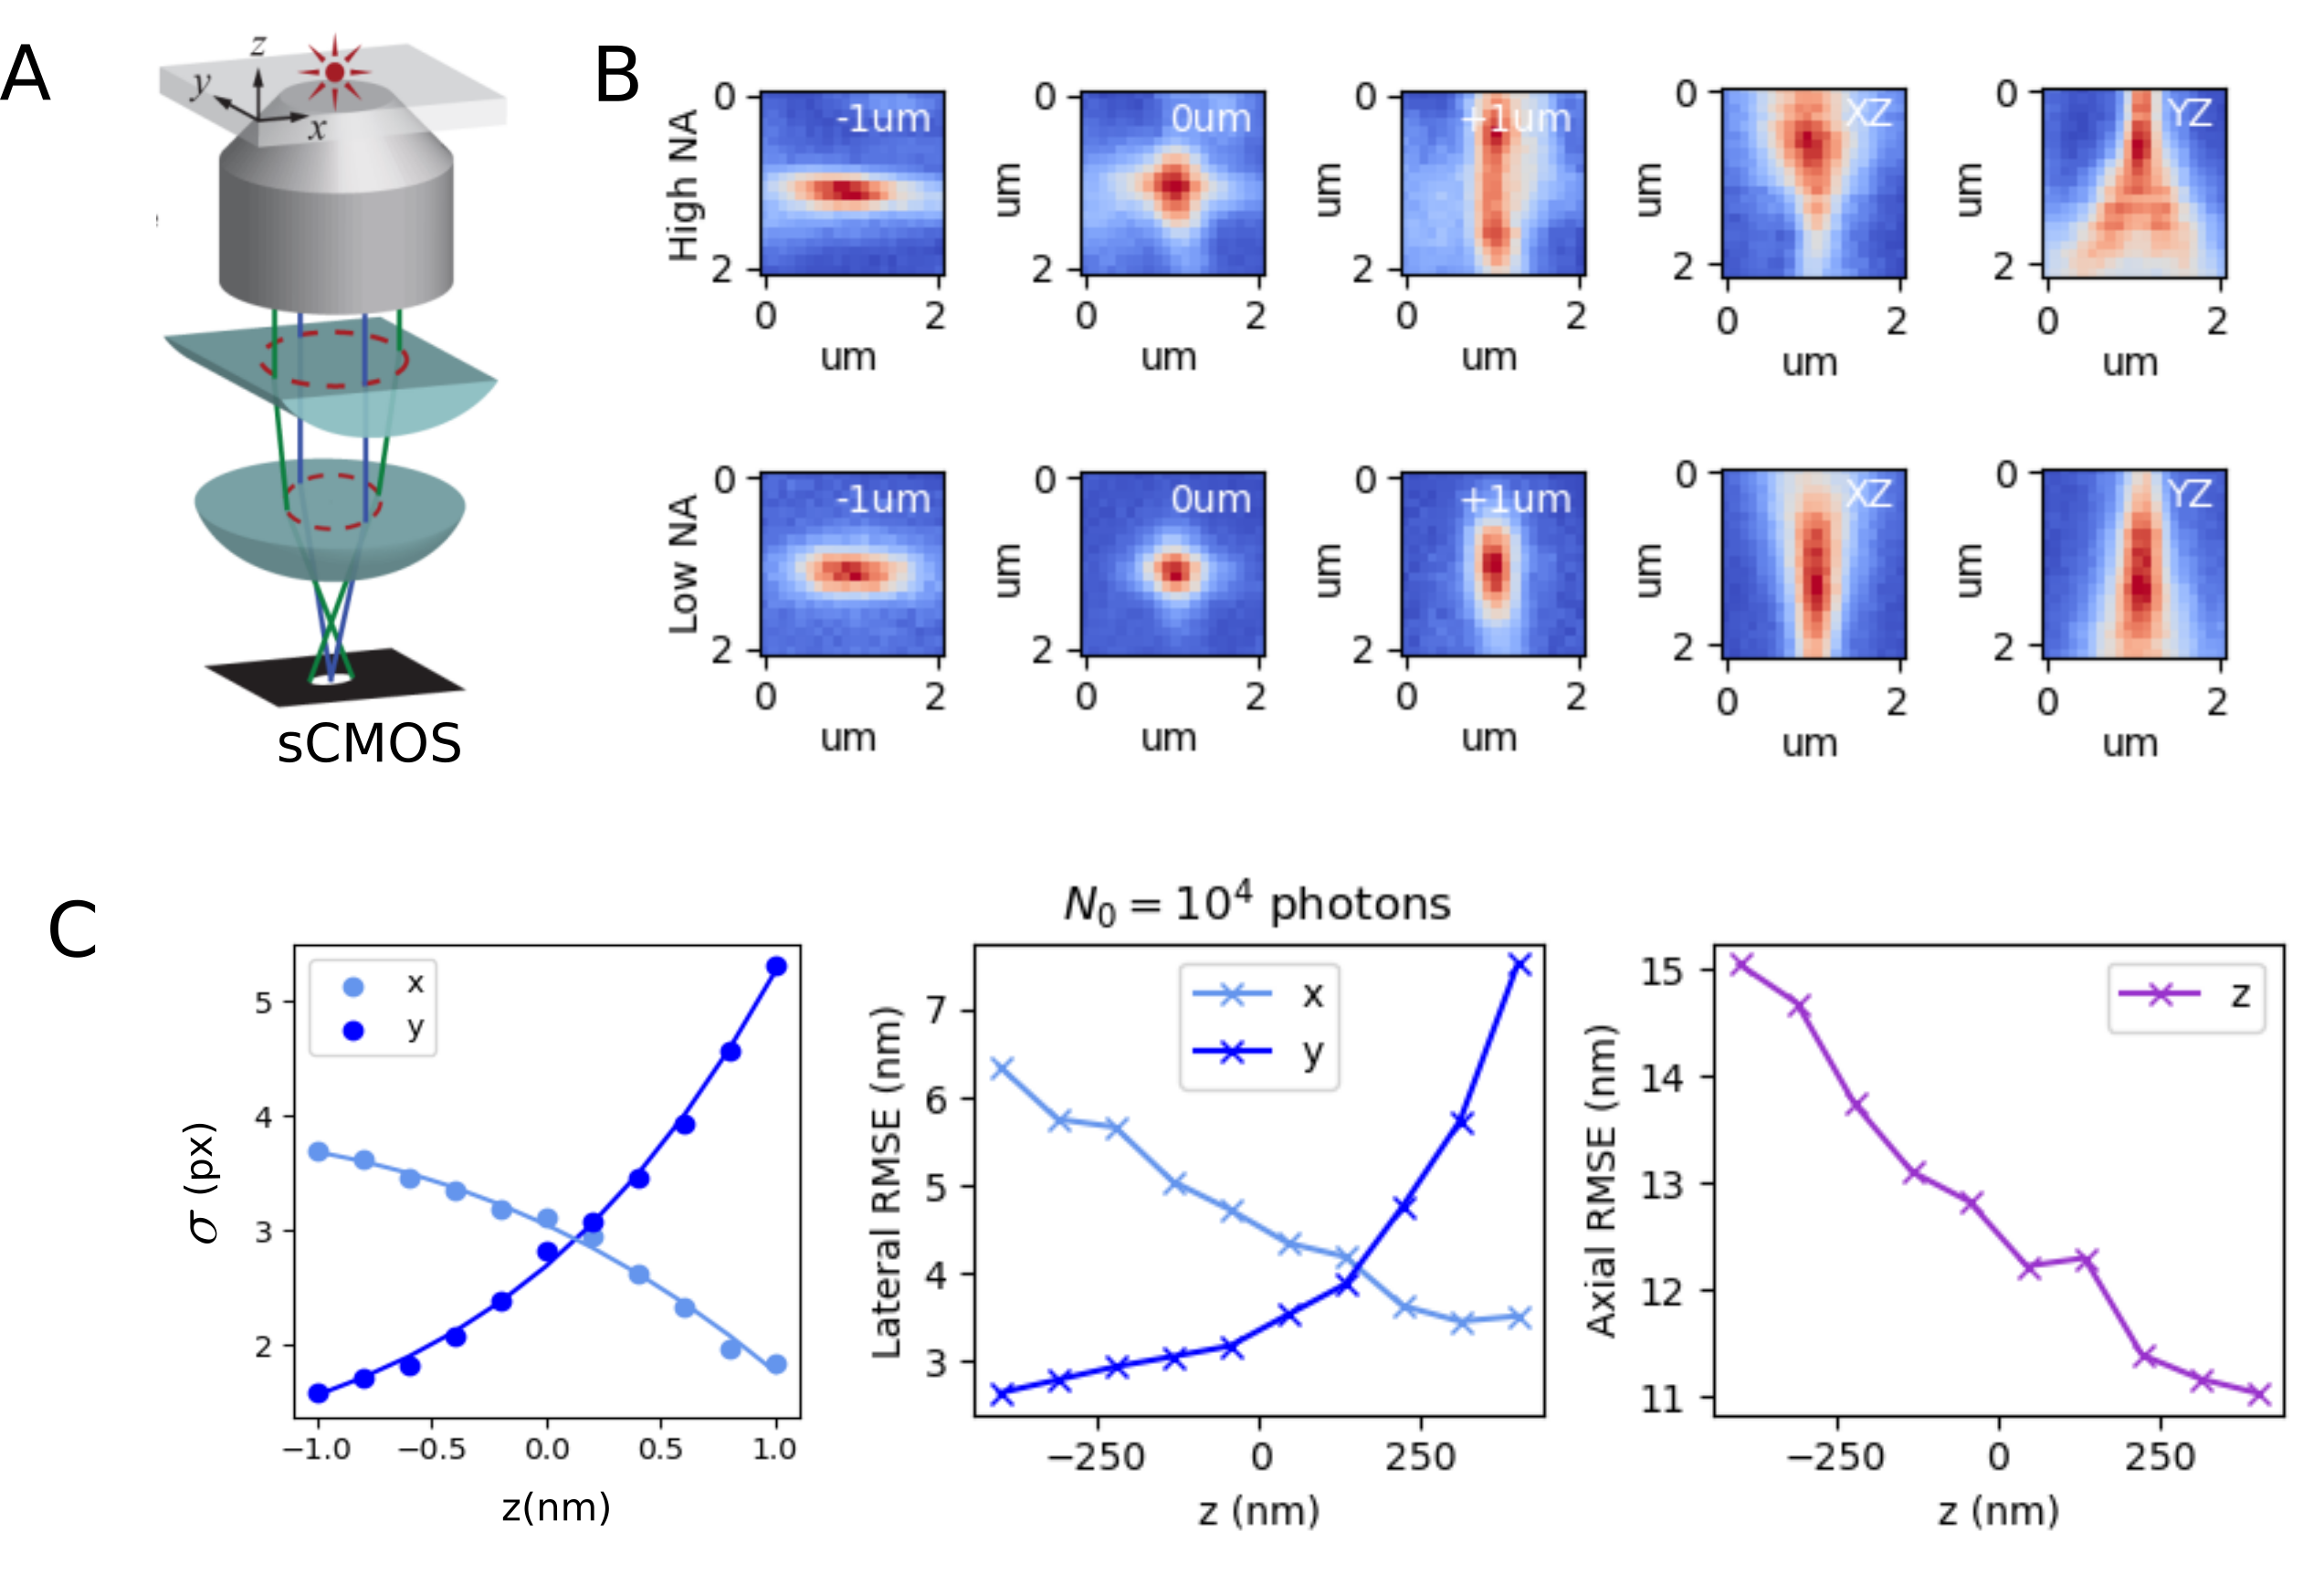
\includegraphics[width=11cm]{Astigmatism.png}
\end{figure}
\begin{itemize}
\item A weak ($f=10$m) cylindrical lens breaks the axial symmetry of the PSF
\end{itemize}
\end{frame}


\begin{frame}{Astigmatism based three dimensional imaging}
\begin{figure}
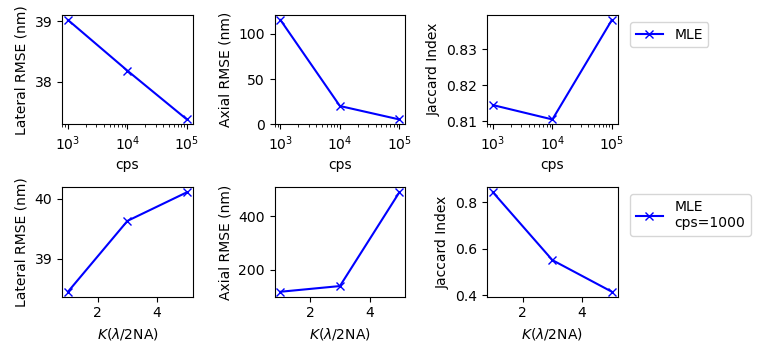
\includegraphics[width=13cm]{PSF3D.png}
\end{figure}
\begin{itemize}
\item $z_{0}\sim U([-0.4,0.4])$ um
\item 3D imaging requires long exposure and sparse emitters for MLE
\item Deep methods may be a suitable choice in future work
\end{itemize}
\end{frame}


\begin{frame}{Chromatin nanodomains in a living Hela cell nucleus}

\begin{textblock*}{13cm}(0.5cm,1.5cm)
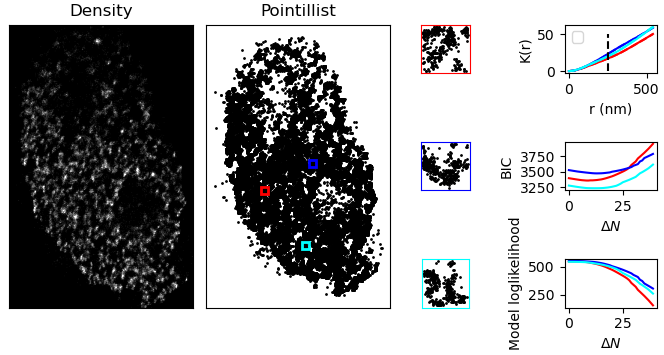
\includegraphics[width=\textwidth]{Cluster.png}
\end{textblock*}

\begin{textblock*}{13cm}(0.5cm,8.0cm)
\begin{itemize}
\item Density estimation using 30x30nm bins
\item Closest pairs are merged one at a time, until we minimized the BIC
\item Data likelihood is computed under a Gaussian Mixture Model (GMM)
\end{itemize}
\end{textblock*}

\end{frame}

\begin{frame}{Chromatin nanodomains in a living Hela cell nucleus}

\begin{textblock*}{13cm}(0.5cm,1.5cm)
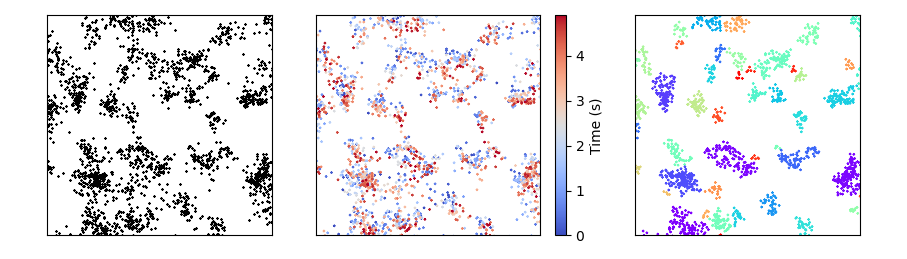
\includegraphics[width=\textwidth]{Cluster2.png}
\end{textblock*}

\begin{textblock*}{13cm}(0.5cm,6.0cm)
\begin{itemize}
\item Density estimation using 30x30nm bins
\item Closest pairs are merged one at a time, until we minimized the BIC
\item Data likelihood is computed under a Gaussian Mixture Model (GMM)
\end{itemize}
\end{textblock*}

\end{frame}




\begin{frame}
\frametitle{}
\centering
\Large \textcolor{black}{Results and Future Aims}
\end{frame}


\begin{frame}{Dissolving BRD4 condensates with JQ1 and 1,6 Hexanediol}
\begin{figure}
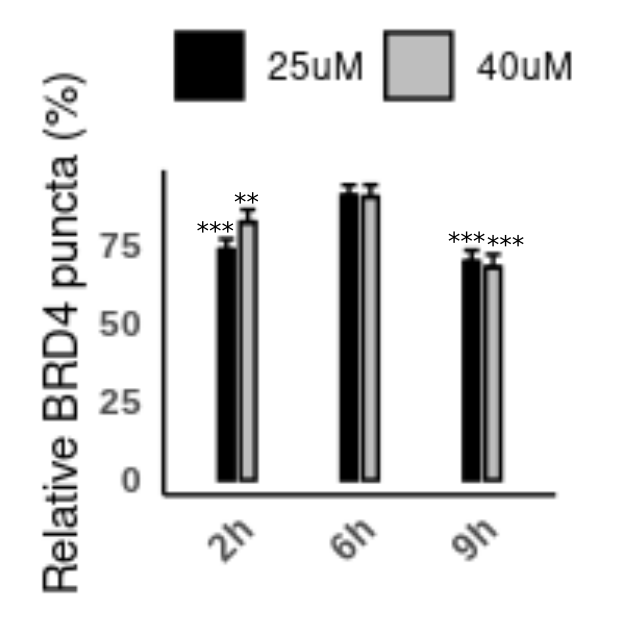
\includegraphics[width=5cm]{BRD4-JQ1.png}
\end{figure}
\end{frame}

\begin{frame}{}
Proposed two and three color imaging experiments
\end{frame}

\begin{frame}{Deep generative modeling with nonequilibrium thermodynamics}
\begin{figure}
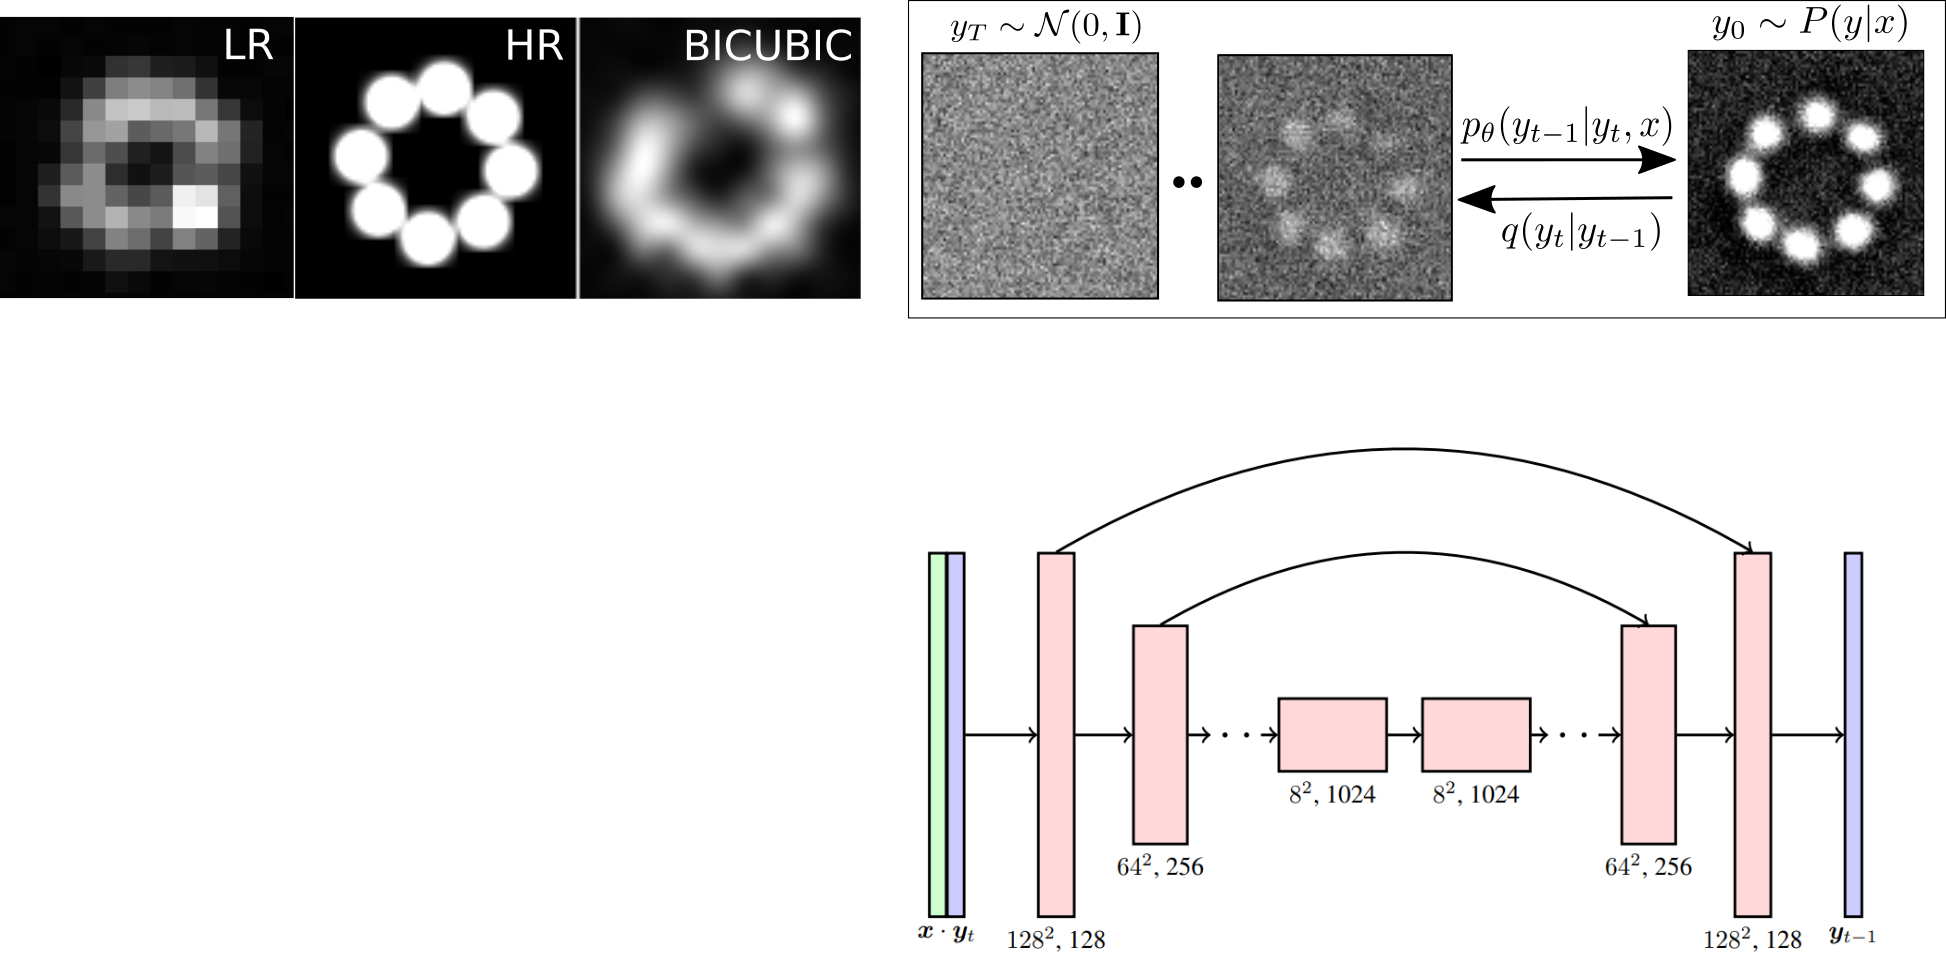
\includegraphics[width=12cm]{Diffusion.png}
\end{figure}
\end{frame}


\begin{frame}{Deep generative modeling with nonequilibrium thermodynamics}
\begin{figure}
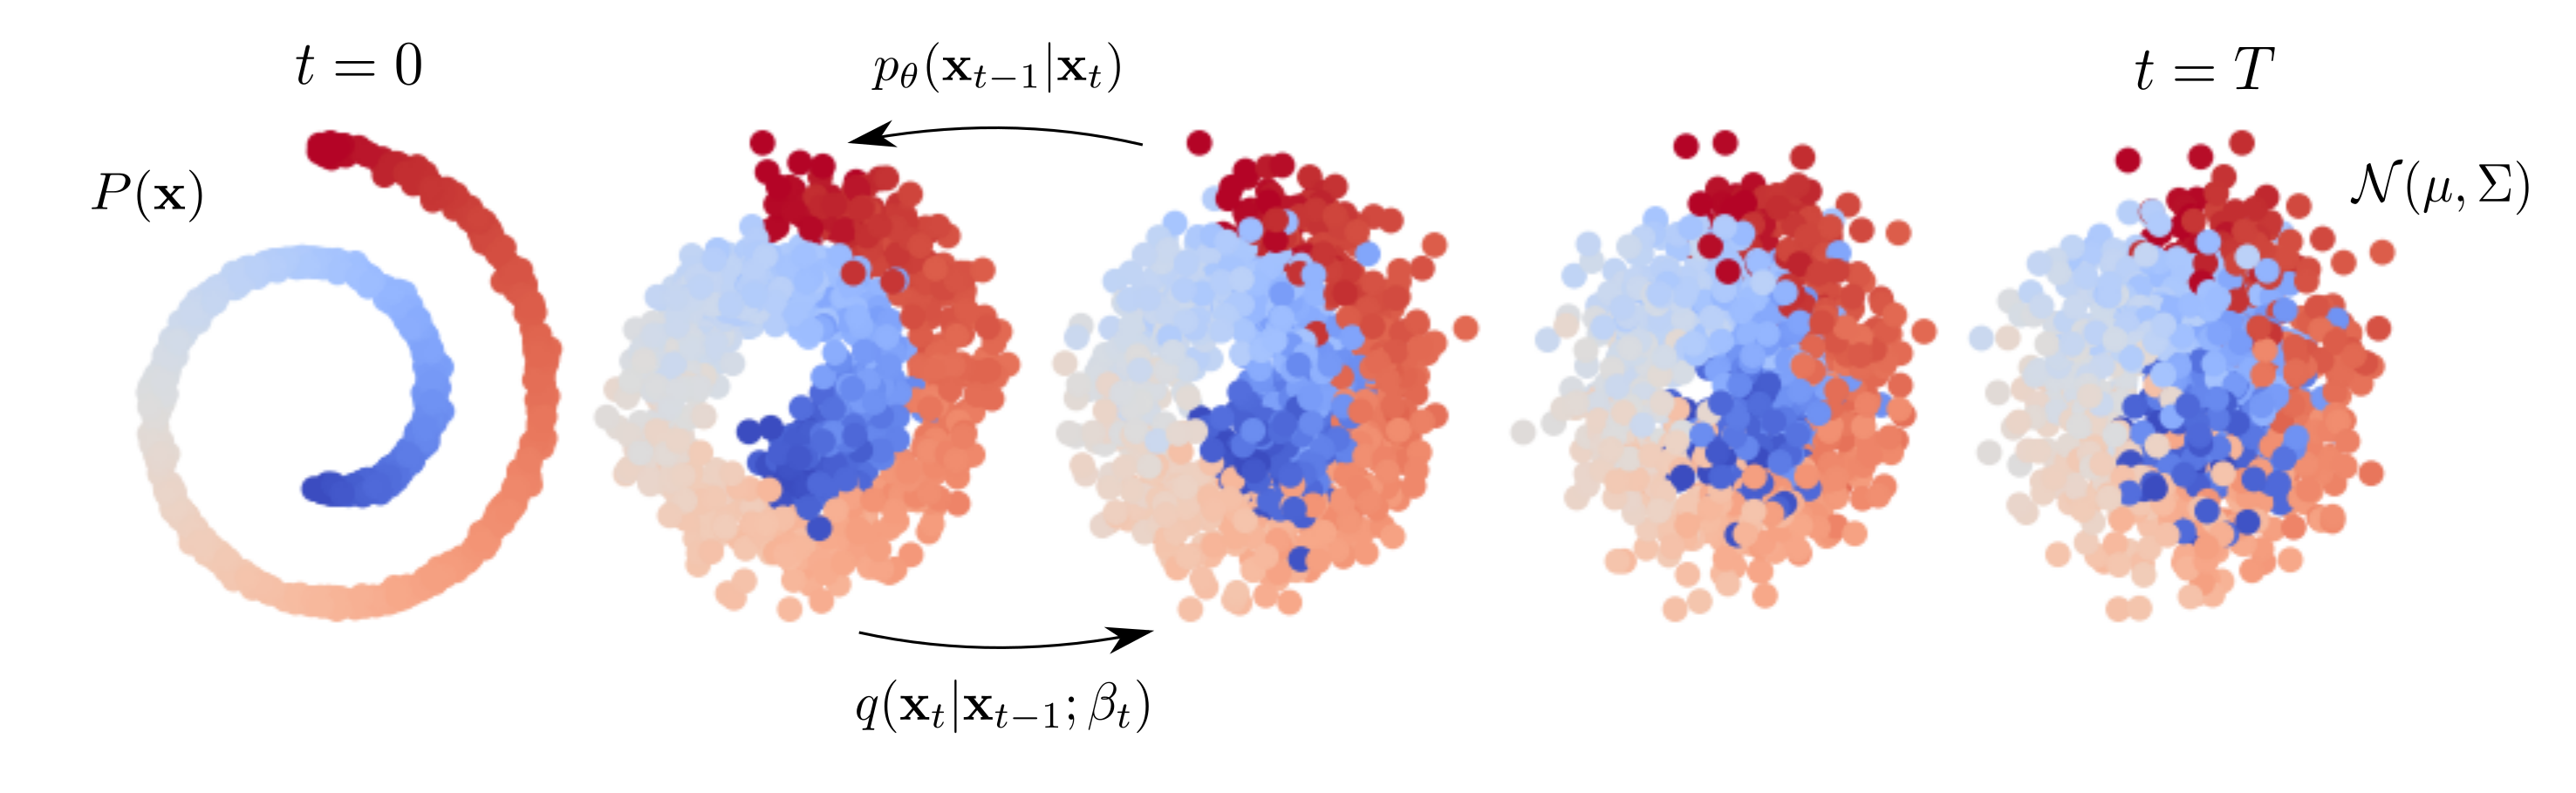
\includegraphics[width=12cm]{DiffusionSwiss.png}
\end{figure}
\begin{itemize}
\item The data distribution is gradually converted into a analytically tractable distributon e.g., Gaussian
\item Repeated application of a Markov transition kernel destroys data structure
\item Use deep neural networks to learn to "reverse time"
\end{itemize}
\end{frame}


\end{document}